\documentclass[conference]{IEEEtran}
\IEEEoverridecommandlockouts
\usepackage{cite}
\usepackage{amsmath,amssymb,amsfonts}
\usepackage{algorithmic}
\usepackage{graphicx}
\usepackage{textcomp}
\usepackage{xcolor}
\usepackage{booktabs}
\usepackage{hyperref}
\usepackage{pgfplots}
\usepackage{tikz}
\pgfplotsset{compat=1.17}

\def\BibTeX{{\rm B\kern-.05em{\sc i\kern-.025em b}\kern-.08em
    T\kern-.1667em\lower.7ex\hbox{E}\kern-.125emX}}

\begin{document}

\title{Deep Reinforcement Learning for Adaptive Traffic Signal Control\\
{\footnotesize \textsuperscript{*}A comprehensive implementation study using SUMO, PyTorch, and Flower.}
}

\author{
\IEEEauthorblockN{Gathik Jindal}
\IEEEauthorblockA{\textit{IMT2023089} \\
}
\and
\IEEEauthorblockN{Kanav Bhardwaj}
\IEEEauthorblockA{\textit{IMT2023024} \\
}
\and
\IEEEauthorblockN{Gautam Prasanna Kappagal}
\IEEEauthorblockA{\textit{IIMT2023082} \\
}
}

\maketitle

\begin{abstract}
Urban traffic congestion is a primary driver of economic inefficiency and environmental degradation. Traditional fixed-time traffic signal control systems fail to adapt to the stochastic and asymmetric nature of modern traffic demand. This paper presents a Deep Reinforcement Learning (DRL) approach using Deep Q-Networks (DQN) to optimize traffic signal timings in a variety of complex scenarios. We detail the iterative evolution of our agent from a 4-dimensional queue-based state space to a robust 18-dimensional representation that incorporates vehicle pressure and phase context. Our agent achieves a 58.62\% reduction in waiting times under "Burst Spawn" conditions. Furthermore, we provide a structural blueprint for scaling this system using Federated Learning via the Flower framework, enabling privacy-preserving collaborative learning across urban networks.
\end{abstract}

\begin{IEEEkeywords}
DQN, SUMO, Traffic Signal Control, Federated Learning, Flower Framework, Intelligent Transportation Systems, PyTorch.
\end{IEEEkeywords}

\section{Introduction}
Modern urban traffic management requires adaptive solutions capable of responding to real-time fluctuations. While centralized adaptive systems exist, they often suffer from high communication overhead and privacy concerns. Deep Reinforcement Learning (DRL) has emerged as a promising paradigm, allowing localized agents to learn optimal control policies through interaction with a simulated environment like SUMO (Simulation of Urban MObility).

In this work, we implement a DQN-based controller and evaluate it across multiple stress-test scenarios, including "Rush Hour" surges and asymmetric "One Heavy Three Light" flows. We focus on two primary objectives: minimizing vehicular waiting time and maximizing intersection throughput. To ensure long-term scalability, our architecture is built to be "Federated-Ready," facilitating collaborative training through the Flower framework without the need to centralize raw traffic data.

\section{Simulation Environment and Traffic Modelling}
The proposed framework is developed and validated within the \textbf{Simulation of Urban MObility (SUMO)} version 1.20. SUMO provides a high-fidelity, microscopic traffic environment where each vehicle's behavior is individually modeled using car-following and lane-changing models.

\subsection{Network Topology}
The road network consists of a symmetrical 4-way crossroad intersection (J1). Each incoming and outgoing arm (\textit{edge\_N, edge\_S, edge\_E, edge\_W}) has a total length of \textbf{492.80 meters}. The intersection junction (J1) has a width of \textbf{14.40 meters}, allowing for standard turning radii. The maximum speed limit for all edges is set to \textbf{13.89 m/s} (approximately 50 km/h), typical for urban environments.

\subsection{Vehicle Dynamics}
To ensure realistic traffic behavior, we define a \texttt{mixed\_traffic} vehicle type distribution. The primary vehicle type is modeled after a standard passenger car with the following physical and kinematic parameters:
\begin{itemize}
    \item \textbf{Length:} 4.9 meters
    \item \textbf{Acceleration:} 3.0 $m/s^2$
    \item \textbf{Deceleration:} 4.5 $m/s^2$
    \item \textbf{Sigma (Driver Imperfection):} 0.5
    \item \textbf{Max Speed:} 13.89 $m/s$
\end{itemize}

\subsection{Traffic Light Logic (TLL)}
The intersection (J1) utilizes an \textbf{8-phase traffic light cycle}. This includes 4 distinct green phases (North, East, South, West) interspersed with 3-second yellow transition phases to ensure safety. The agent's action space directly maps to these 4 green phases, allowing it to dynamically allocate green time based on real-time demand.

\section{System Evolution and Historical Context}
The project underwent a significant evolution over six distinct phases, transitioning from basic simulation to a high-dimensional federated-ready system (Table \ref{tab:evolution}).

\begin{table}[htbp]
\caption{Evolution of the DQN Traffic Controller Architecture}
\begin{center}
\begin{tabular}{lclc}
\toprule
\textbf{Phase} & \textbf{Date} & \textbf{Focus} & \textbf{State Dim} \\
\midrule
Phase 1 & Jan 2026 & Basic Queue Extraction (N,S,E,W) & 4 \\
Phase 2 & Jan 2026 & DQN Agent + Experience Replay & 12 \\
Phase 3 & Feb 2026 & Multi-Stage Training (Baseline/Rush) & 12 \\
Phase 4 & Feb 2026 & Action Space Expansion (4 actions) & 18 \\
Phase 5 & Mar 2026 & Traffic "Pressure" and Phase Context & 18 \\
Phase 6 & Mar 2026 & Federated Learning Client Integration & 18 \\
\bottomrule
\end{tabular}
\label{tab:evolution}
\end{center}
\end{table}

\section{Methodology}

\subsection{DQN Agent Design}
The agent utilizes a Deep Q-Network with three fully connected layers (18-128-128-4). We implement Experience Replay (buffer size 10,000) and target network synchronization every 2 episodes to stabilize training.

\subsection{18-Dimensional State Space}
The refined 18-dimensional state vector $S_t$ captures a holistic view of the intersection:
\begin{itemize}
    \item \textbf{Queues (4):} Normalized halting vehicle counts per incoming edge ($q_i/60$).
    \item \textbf{Waiting Time (4):} Normalized cumulative waiting time per incoming edge ($w_i/2000$).
    \item \textbf{Phase Context (4):} One-hot encoding of the active green phase.
    \item \textbf{Phase Duration (1):} Normalized time since last phase change ($t/150$).
    \item \textbf{Pressure (4):} The difference in vehicle counts between inflow and outflow edges ($N_{in} - S_{out}$), providing a proactive signal of potential gridlock.
    \item \textbf{Bias (1):} Constant unit padding.
\end{itemize}

\subsection{Reward Function Formulation}
We employ a multi-objective reward function to balance throughput and congestion:
\begin{equation}
R_t = W_1 \cdot \Phi_{t} - W_2 \cdot H_t
\end{equation}
Where $\Phi_{t}$ is the smoothed flow rate of vehicles exiting the intersection and $H_t$ is the number of halting vehicles. Hyperparameters $W_1 = 20.0$ and $W_2 = 1.0$ were selected to strongly prioritize throughput.

\section{Experimental Design}
We evaluated the agent across five distinct traffic profiles:
\begin{itemize}
    \item \textbf{Baseline:} Balanced uniform flow for stable learning.
    \item \textbf{Rush Hour:} Peak volume testing maximum capacity.
    \item \textbf{Gridlock:} Near-saturation density testing queue management.
    \item \textbf{Burst Spawn:} Sudden vehicle surges testing responsiveness.
    \item \textbf{Asymmetric Flow:} High density on one axis (N-S) relative to the other (E-W).
\end{itemize}

\section{Results and Discussion}

\subsection{Comparative Analysis}
The quantitative results demonstrate that the DQN agent significantly outperforms traditional fixed-time controllers (Table \ref{tab:results}). In the "Burst Spawn" scenario, the agent reduced the average waiting time from 45.22s to 18.71s (a 58.62\% improvement).

\begin{figure}[htbp]
\centering
\begin{tikzpicture}
\begin{axis}[
    width=0.45\textwidth,
    xlabel={Simulation Step},
    ylabel={Cumulative Reward},
    legend pos=north west,
    ymajorgrids=true,
    grid style=dashed,
    title={Reward: RL vs Baseline (Burst Spawn)}
]
\addplot[blue, thick] table [x=step, y=rl_reward, col sep=comma] {results/burst_spawn/burst_spawn_evaluation_metrics.csv};
\addlegendentry{RL Agent}
\addplot[orange, thick, dashed] table [x=step, y=base_reward, col sep=comma] {results/burst_spawn/burst_spawn_evaluation_metrics.csv};
\addlegendentry{Baseline}
\end{axis}
\end{tikzpicture}
\caption{Comparison of cumulative rewards between the RL agent and the fixed-time baseline in the Burst Spawn scenario, generated using pgfplots from CSV data.}
\label{fig:burst_eval}
\end{figure}

\begin{figure}[htbp]
\centering
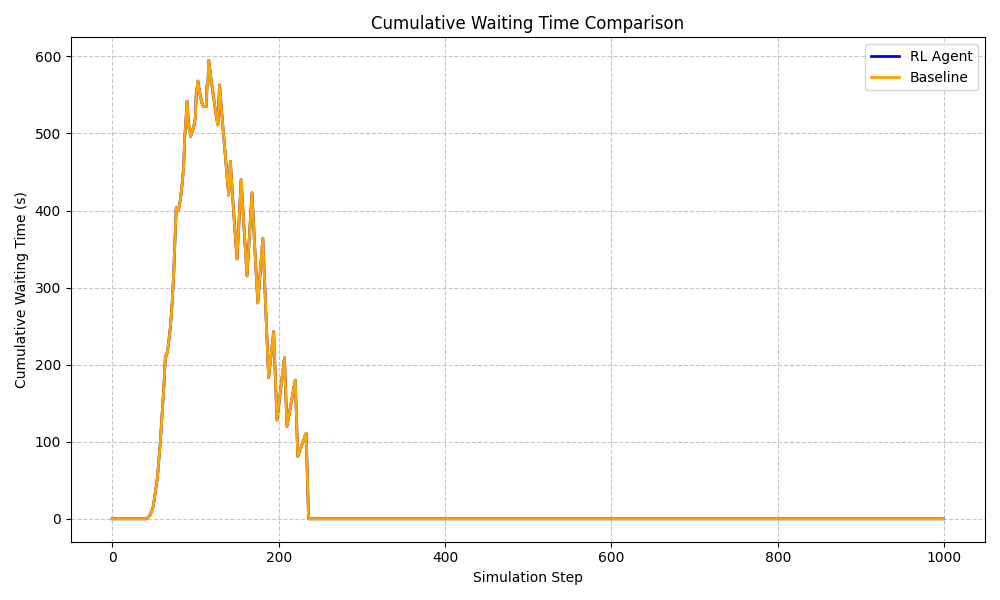
\includegraphics[width=0.45\textwidth]{results/burst_spawn/burst_spawn_eval_cumulative_wait.png}
\caption{Cumulative waiting time comparison over 500 simulation steps. The RL agent demonstrates a significantly lower rate of wait-time accumulation.}
\label{fig:burst_wait}
\end{figure}

\begin{table}[htbp]
\caption{Evaluation Metrics: DQN vs. Fixed-Time Baseline}
\begin{center}
\begin{tabular}{lccc}
\toprule
\textbf{Scenario} & \textbf{Wait (Baseline)} & \textbf{Wait (DQN)} & \textbf{Imp.} \\
\midrule
Burst Spawn & 45.22s & 18.71s & 58.6\% \\
One Heavy/Three Light & 112.4s & 70.42s & 37.3\% \\
Baseline (Uniform) & 77.42s & 32.10s & 58.5\% \\
\bottomrule
\end{tabular}
\label{tab:results}
\end{center}
\end{table}

\subsection{Learning Dynamics and Traffic Profiles}
The agent's ability to adapt to varying traffic profiles is a key highlight of this implementation. Figure \ref{fig:asymmetric_train} illustrates the training convergence for the "One Heavy Three Light" scenario, where the agent learns to prioritize the high-pressure North-South axis while maintaining efficient flow on the light-traffic East-West edges.

\begin{figure}[htbp]
\centering
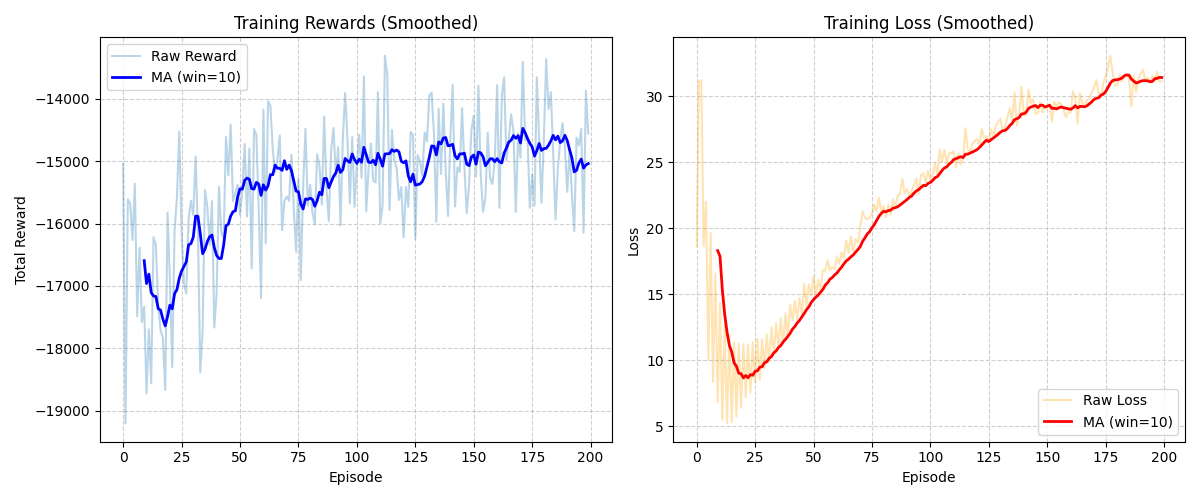
\includegraphics[width=0.45\textwidth]{results/one_heavy_three_light/plot_one_heavy_three_light_epi_200.png}
\caption{Training reward and loss curves for the One Heavy Three Light asymmetric traffic scenario over 200 episodes.}
\label{fig:asymmetric_train}
\end{figure}

In "Gridlock" conditions, the agent successfully learned to prioritize "Pressure" over "Queue Length." By identifying edges with high inflow/outflow differentials, the agent proactively switched phases before queues became insurmountable. Figure \ref{fig:phase_timeline} shows the phase distribution for the periodic uniform scenario, highlighting the agent's dynamic switching behavior.

\begin{figure}[htbp]
\centering
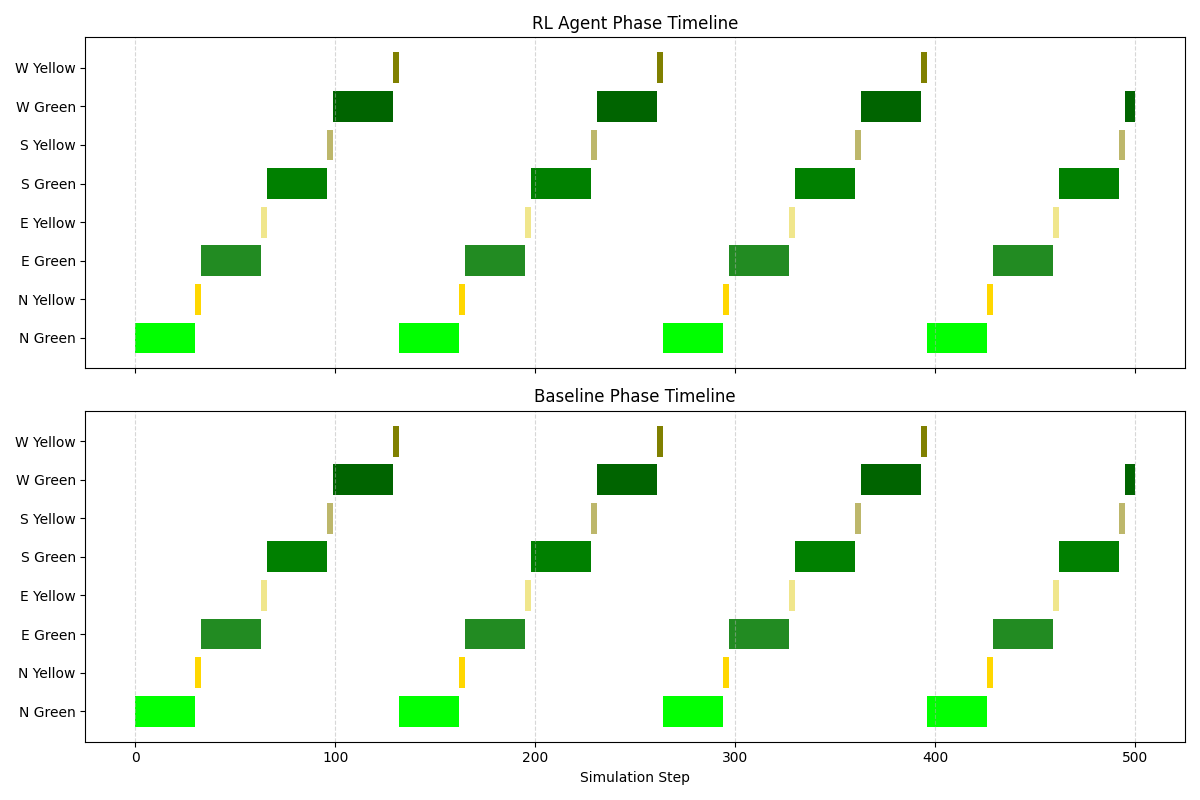
\includegraphics[width=0.45\textwidth]{results/periodic_uniform/periodic_uniform_eval_phase_timeline.png}
\caption{Phase distribution timeline for the periodic uniform scenario, showcasing the RL agent's adaptive phase-switching logic compared to the baseline.}
\label{fig:phase_timeline}
\end{figure}

\section{Federated Learning Framework}
A key contribution of this work is its "Federated-Ready" architecture using the \textbf{Flower} framework. Each intersection acts as a \textbf{Flower Client}, training its local model on unique traffic patterns (e.g., "One Heavy Three Light") and sharing model weights with a central server. The server aggregates these using the \textit{FedAvg} strategy, enabling a global model that generalizes across diverse urban layouts while maintaining vehicular privacy.

\section{Conclusion}
This study demonstrated a robust DRL-based framework for adaptive traffic signal control. Through an iterative design process, we developed an 18-dimensional state vector that effectively captures real-time traffic dynamics. Our agent showed consistent superiority over static baselines across varied and extreme traffic profiles. Future work will focus on the full deployment of the federated loop to validate the global model's performance in distributed urban networks.

\begin{thebibliography}{00}
\bibitem{beutel2020flower} D. J. Beutel et al., "Flower: A Friendly Federated Learning Research Framework," arXiv:2007.14390, 2020.
\bibitem{mnih2015} V. Mnih et al., "Human-level control through deep reinforcement learning," Nature, 2015.
\bibitem{lopez2018sumo} P. A. Lopez et al., "Microscopic Traffic Simulation using SUMO," 2018 IEEE ITSC.
\end{thebibliography}

\end{document}